% Compile with: pdflatex multistate-diagram.tex
% Then convert to SVG: pdf2svg multistate-diagram.pdf multistate-diagram.svg
\documentclass[tikz,border=15pt]{standalone}
\usepackage{tikz}
\usetikzlibrary{shapes,arrows.meta,positioning,calc,decorations.markings}
\usepackage{amsmath}
\usepackage{helvet}
\renewcommand{\familydefault}{\sfdefault}
\usepackage{sfmath}

\begin{document}

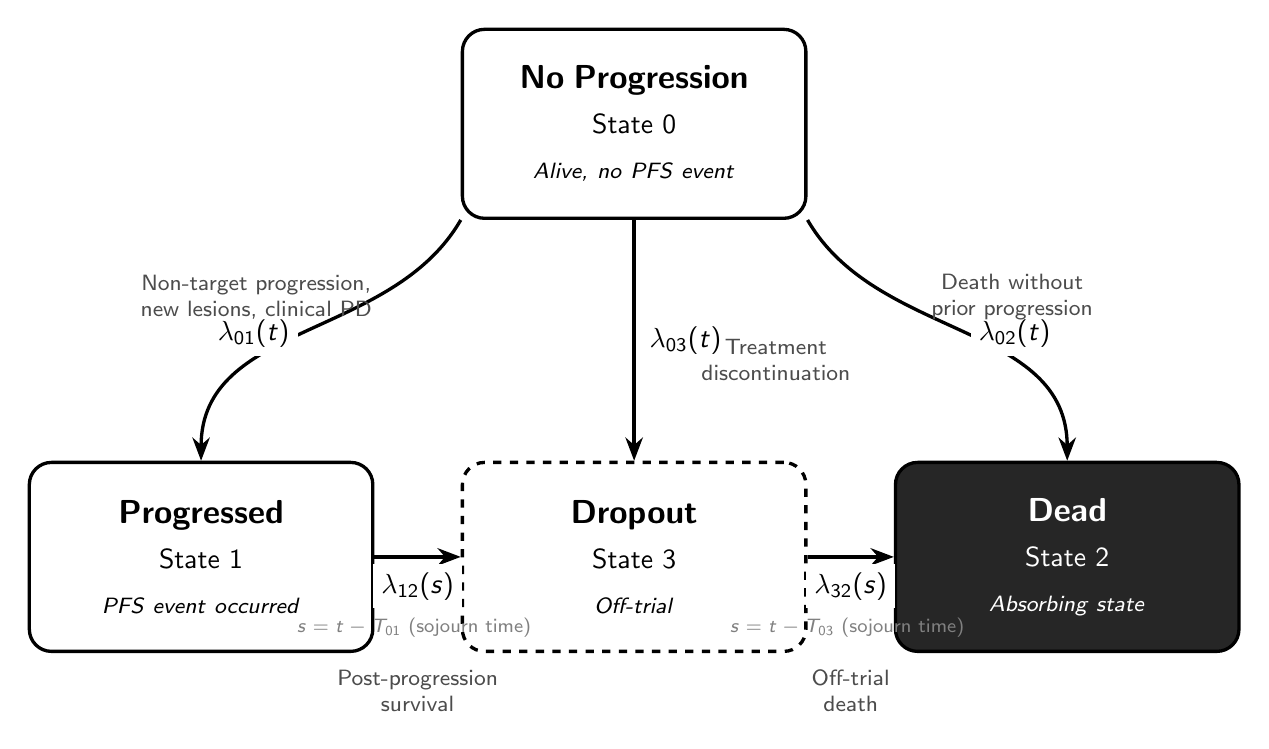
\begin{tikzpicture}[
  state/.style={
    rectangle, rounded corners=8pt,
    minimum width=4.2cm, minimum height=2.4cm,
    text centered, draw=black, line width=1.2pt,
    font=\normalsize, align=center, inner sep=8pt
  },
  transition/.style={
    -Stealth,
    line width=1.2pt, black
  },
  hazlabel/.style={
    font=\normalsize, fill=white, inner sep=3pt
  }
]

% ==================== STATES ====================

% State 0: No Progression (top center)
\node (s0) [state, fill=white, text width=3.8cm] at (0, 0) {
    \large\textbf{No Progression}\\[0.15cm]
    \normalsize State 0\\[0.15cm]
    \footnotesize\textit{Alive, no PFS event}
};

% State 1: Progressed (bottom left)
\node (s1) [state, fill=white, text width=3.8cm] at (-5.5, -5.5) {
    \large\textbf{Progressed}\\[0.15cm]
    \normalsize State 1\\[0.15cm]
    \footnotesize\textit{PFS event occurred}
};

% State 2: Dead (bottom right) - absorbing state
\node (s2) [state, fill=black!85, text=white, text width=3.8cm] at (5.5, -5.5) {
    \large\textbf{Dead}\\[0.15cm]
    \normalsize State 2\\[0.15cm]
    \footnotesize\textit{Absorbing state}
};

% State 3: Dropout (below State 0, between States 1 and 2)
\node (s3) [state, fill=white, text width=3.8cm, dashed] at (0, -5.5) {
    \large\textbf{Dropout}\\[0.15cm]
    \normalsize State 3\\[0.15cm]
    \footnotesize\textit{Off-trial}
};

% ==================== TRANSITIONS ====================

% 0 -> 1: Progression
\draw [transition] (s0.south west) to[out=240,in=90]
    node[hazlabel, pos=0.5, left=2pt] {$\lambda_{01}(t)$}
    (s1.north);

% 0 -> 2: Death without progression
\draw [transition] (s0.south east) to[out=300,in=90]
    node[hazlabel, pos=0.5, right=2pt] {$\lambda_{02}(t)$}
    (s2.north);

% 0 -> 3: Treatment discontinuation (dropout)
\draw [transition] (s0.south) --
    node[hazlabel, pos=0.5, right=2pt] {$\lambda_{03}(t)$}
    (s3.north);

% 1 -> 2: Post-progression death
\draw [transition] (s1.east) --
    node[hazlabel, pos=0.5, below=2pt] {$\lambda_{12}(s)$}
    (s3.west);

% 3 -> 2: Off-trial death
\draw [transition] (s3.east) --
    node[hazlabel, pos=0.5, below=2pt] {$\lambda_{32}(s)$}
    (s2.west);

% ==================== ANNOTATIONS ====================

% Transition descriptions
\node[font=\footnotesize, text=black!70, align=center] at (-4.8, -2.2) {
    Non-target progression,\\new lesions, clinical PD
};

\node[font=\footnotesize, text=black!70, align=center] at (4.8, -2.2) {
    Death without\\prior progression
};

\node[font=\footnotesize, text=black!70, align=center] at (1.8, -3.0) {
    Treatment\\discontinuation
};

\node[font=\footnotesize, text=black!70, align=center] at (-2.75, -7.2) {
    Post-progression\\survival
};

% Time scale note for 1->2
\node[font=\scriptsize, text=black!50, align=center] at (-2.75, -6.4) {
    $s = t - T_{01}$ (sojourn time)
};

\node[font=\footnotesize, text=black!70, align=center] at (2.75, -7.2) {
    Off-trial\\death
};

% Time scale note for 3->2
\node[font=\scriptsize, text=black!50, align=center] at (2.75, -6.4) {
    $s = t - T_{03}$ (sojourn time)
};

\end{tikzpicture}
\end{document}
